%% Requires compilation with XeLaTeX or LuaLaTeX
%% based on UC Berkeley Beamer theme https://www.overleaf.com/latex/templates/uc-berkeley-beamer-theme/bywswngntrws
\documentclass[10pt,xcolor={table,dvipsnames},t]{beamer}

\usetheme{UCBerkeley}
\setbeamertemplate{footline}[frame number] 
\RequirePackage[style=numeric]{biblatex}
\addbibresource{refs.bib}
\RequirePackage{csquotes}
\RequirePackage{amsmath}
\RequirePackage{physics}
\RequirePackage{graphicx}
\RequirePackage[font=small]{caption, subcaption}
\RequirePackage{wrapfig}
\RequirePackage{siunitx}
\RequirePackage{sidecap}
\RequirePackage{caption}
\RequirePackage{booktabs}
\captionsetup[figure]{font = scriptsize, labelfont = scriptsize} % https://tex.stackexchange.com/questions/52132/beamer-change-size-of-figure-caption
\setkeys{Gin}{width=1\linewidth}


\title[Autosailboat]{Autonomous control of a sailboat}
\author{Neelay Junnarkar, Andrew Fearing, Hamza Khawaja}
% \institute{Your Faculty/Department}
\date{\today}

\begin{document}

\begin{frame}
  \titlepage
\end{frame}

\begin{frame}{Outline}
 \tableofcontents
\end{frame}
\section{Introduction}
\begin{frame}{Team}

Neelay Junnarkar

\hfill\\
Andrew Fearing

\hfill\\
Hamza Khawaja
\end{frame}


\begin{frame}{Motivation}
\begin{columns}
\column{0.5\linewidth}
    \begin{figure}
        \centering
        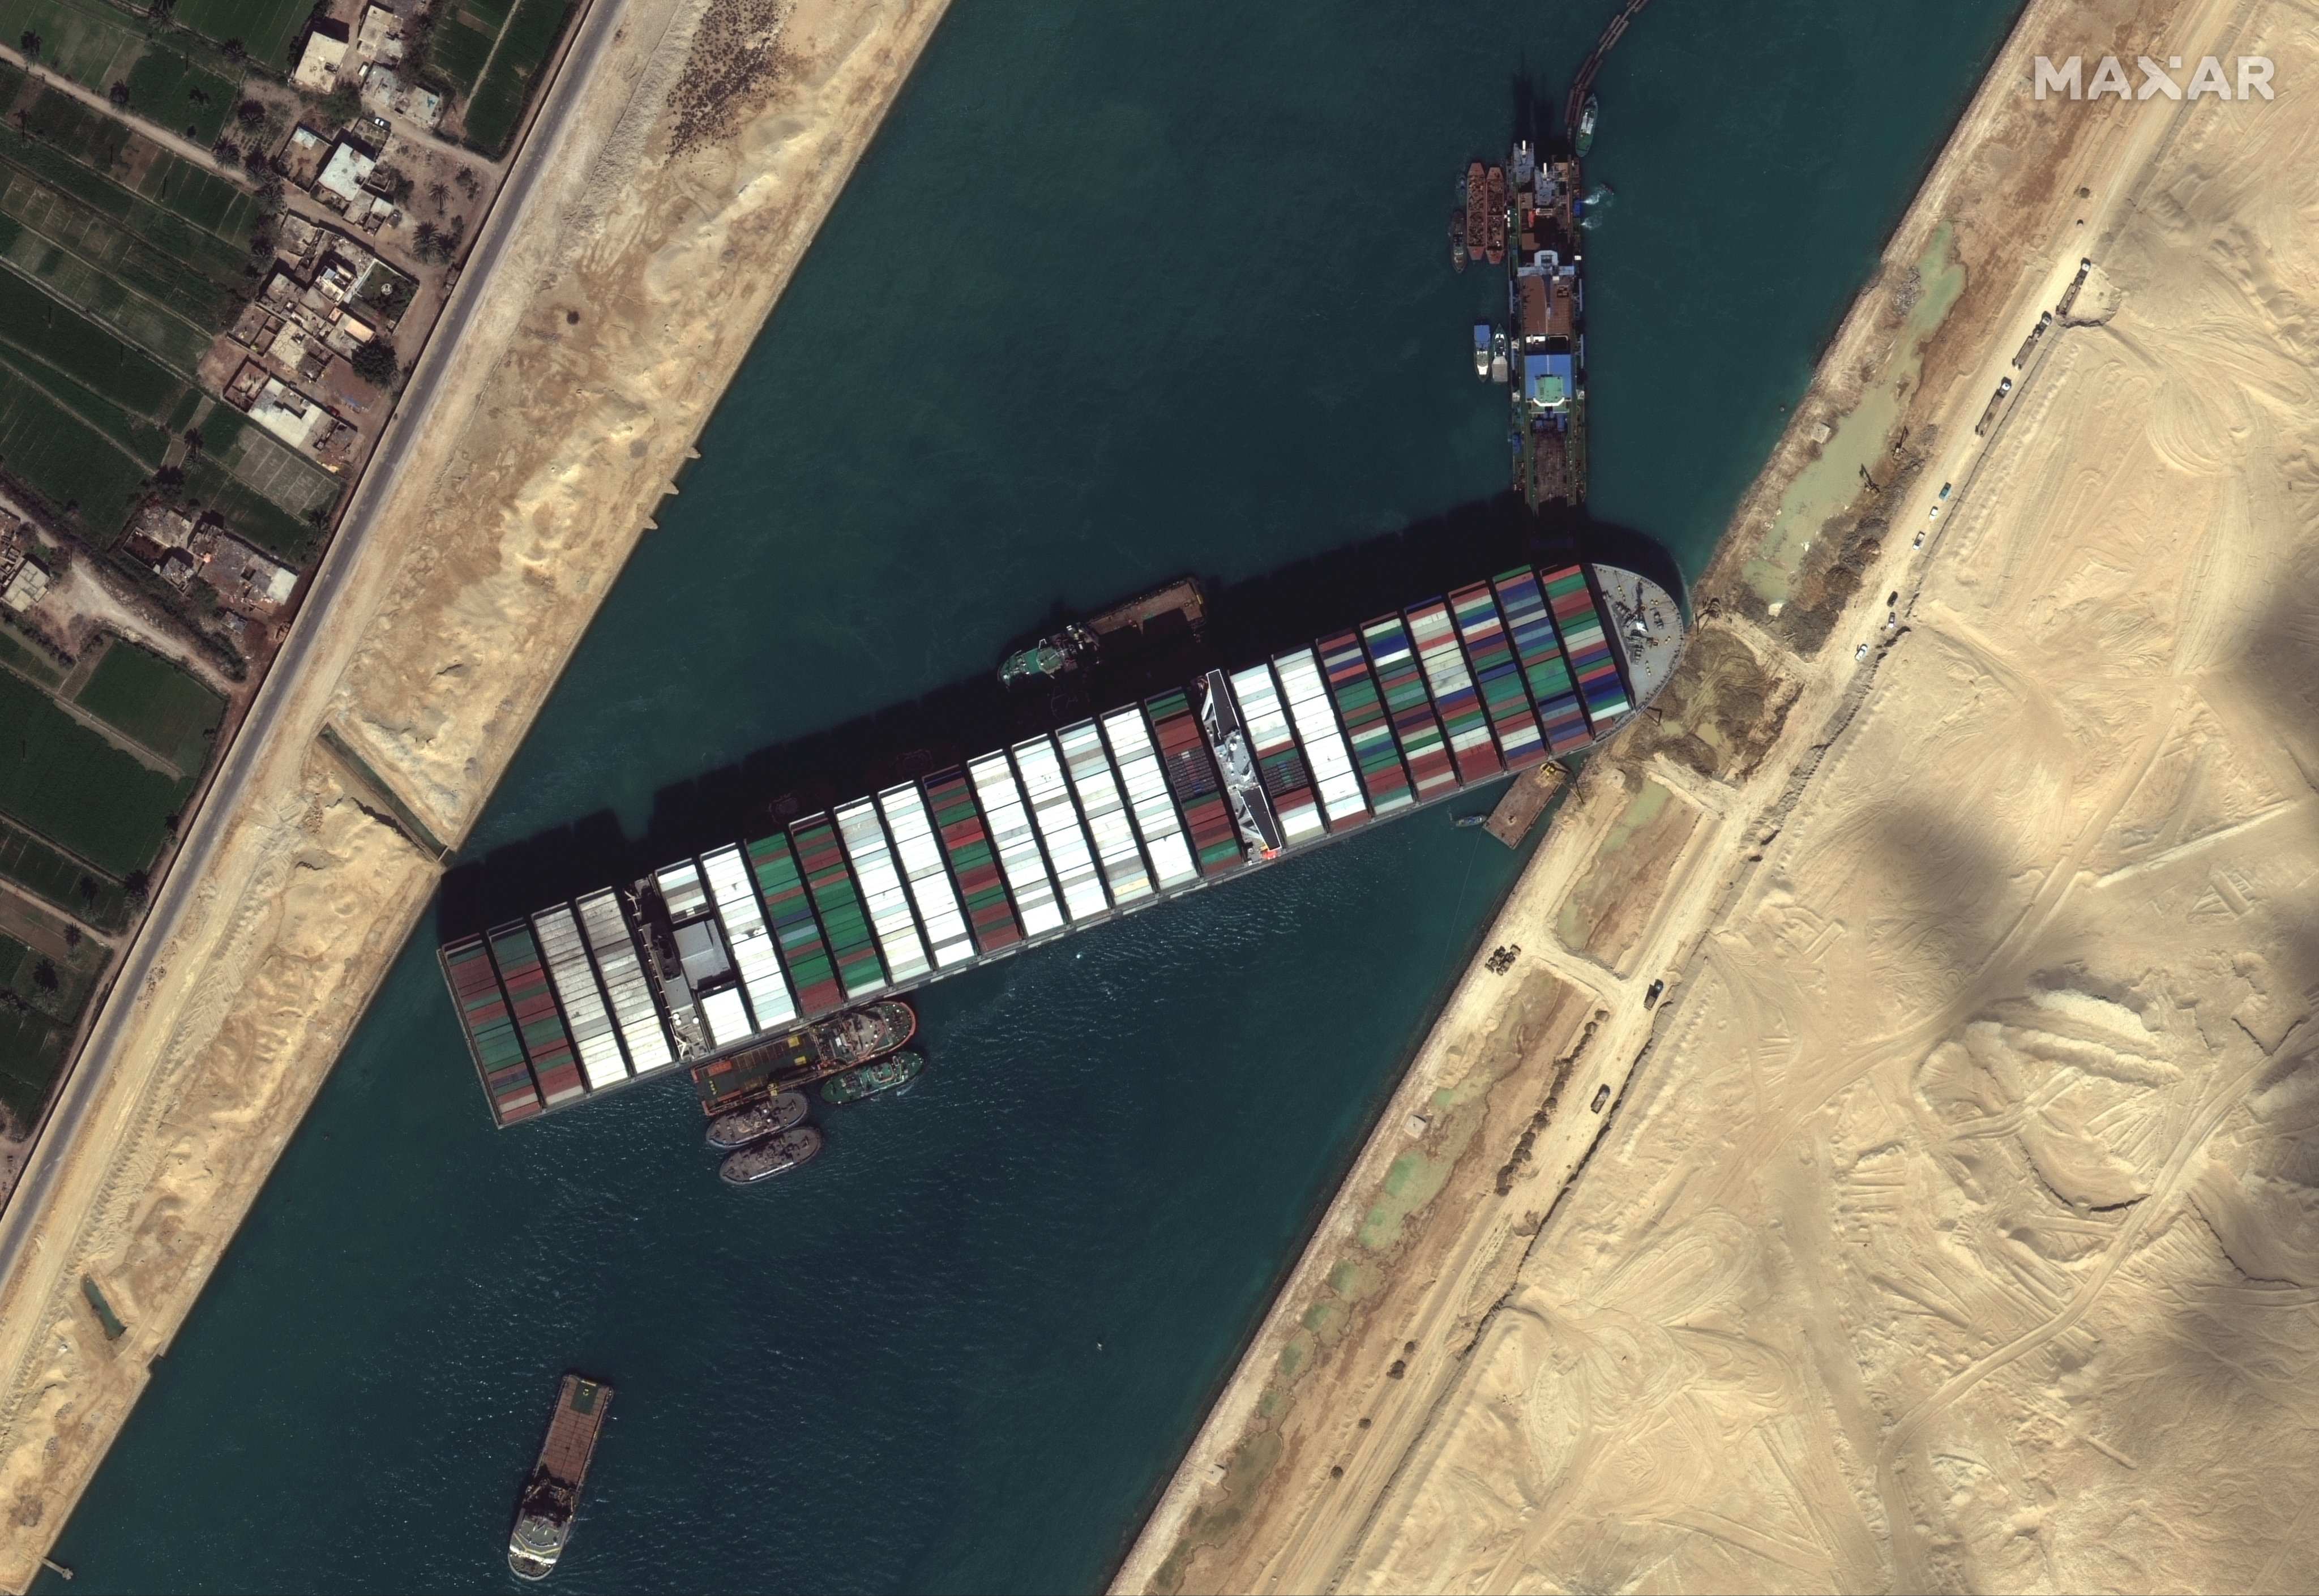
\includegraphics{documents/figures/Suez_Canal_blocked_by_Ever_Given_March_27_2021.jpg}
        \caption{Boat stuck}
        \label{fig:boat_stuck}
    \end{figure}  
\column{0.5\linewidth}
    \textbf{Control of sailboats}
    
    \hfill\\
    Controlling boats autonomously presents an interesting challenge due to the large effect of environmental disturbances such as wind, water currents, and waves. 
    
    \hfill\\
    \textbf{Why Sailboats?}
    
    \hfill\\
    Sailboats are useful for low-power long-term deployments. Also, present a gap in current literature,
    especially in controller design.
    
\end{columns}
\end{frame}

\begin{frame}{Goal}

\begin{enumerate}
    \item Develop sailboat yaw controller.
    \item Develop path planner which can navigate channels.
\end{enumerate}
Focus on robustness to environmental disturbances.

\end{frame}
  

\begin{frame}{Sailing}
\begin{columns}
\column{0.5\linewidth}

\begin{figure}
    \centering
    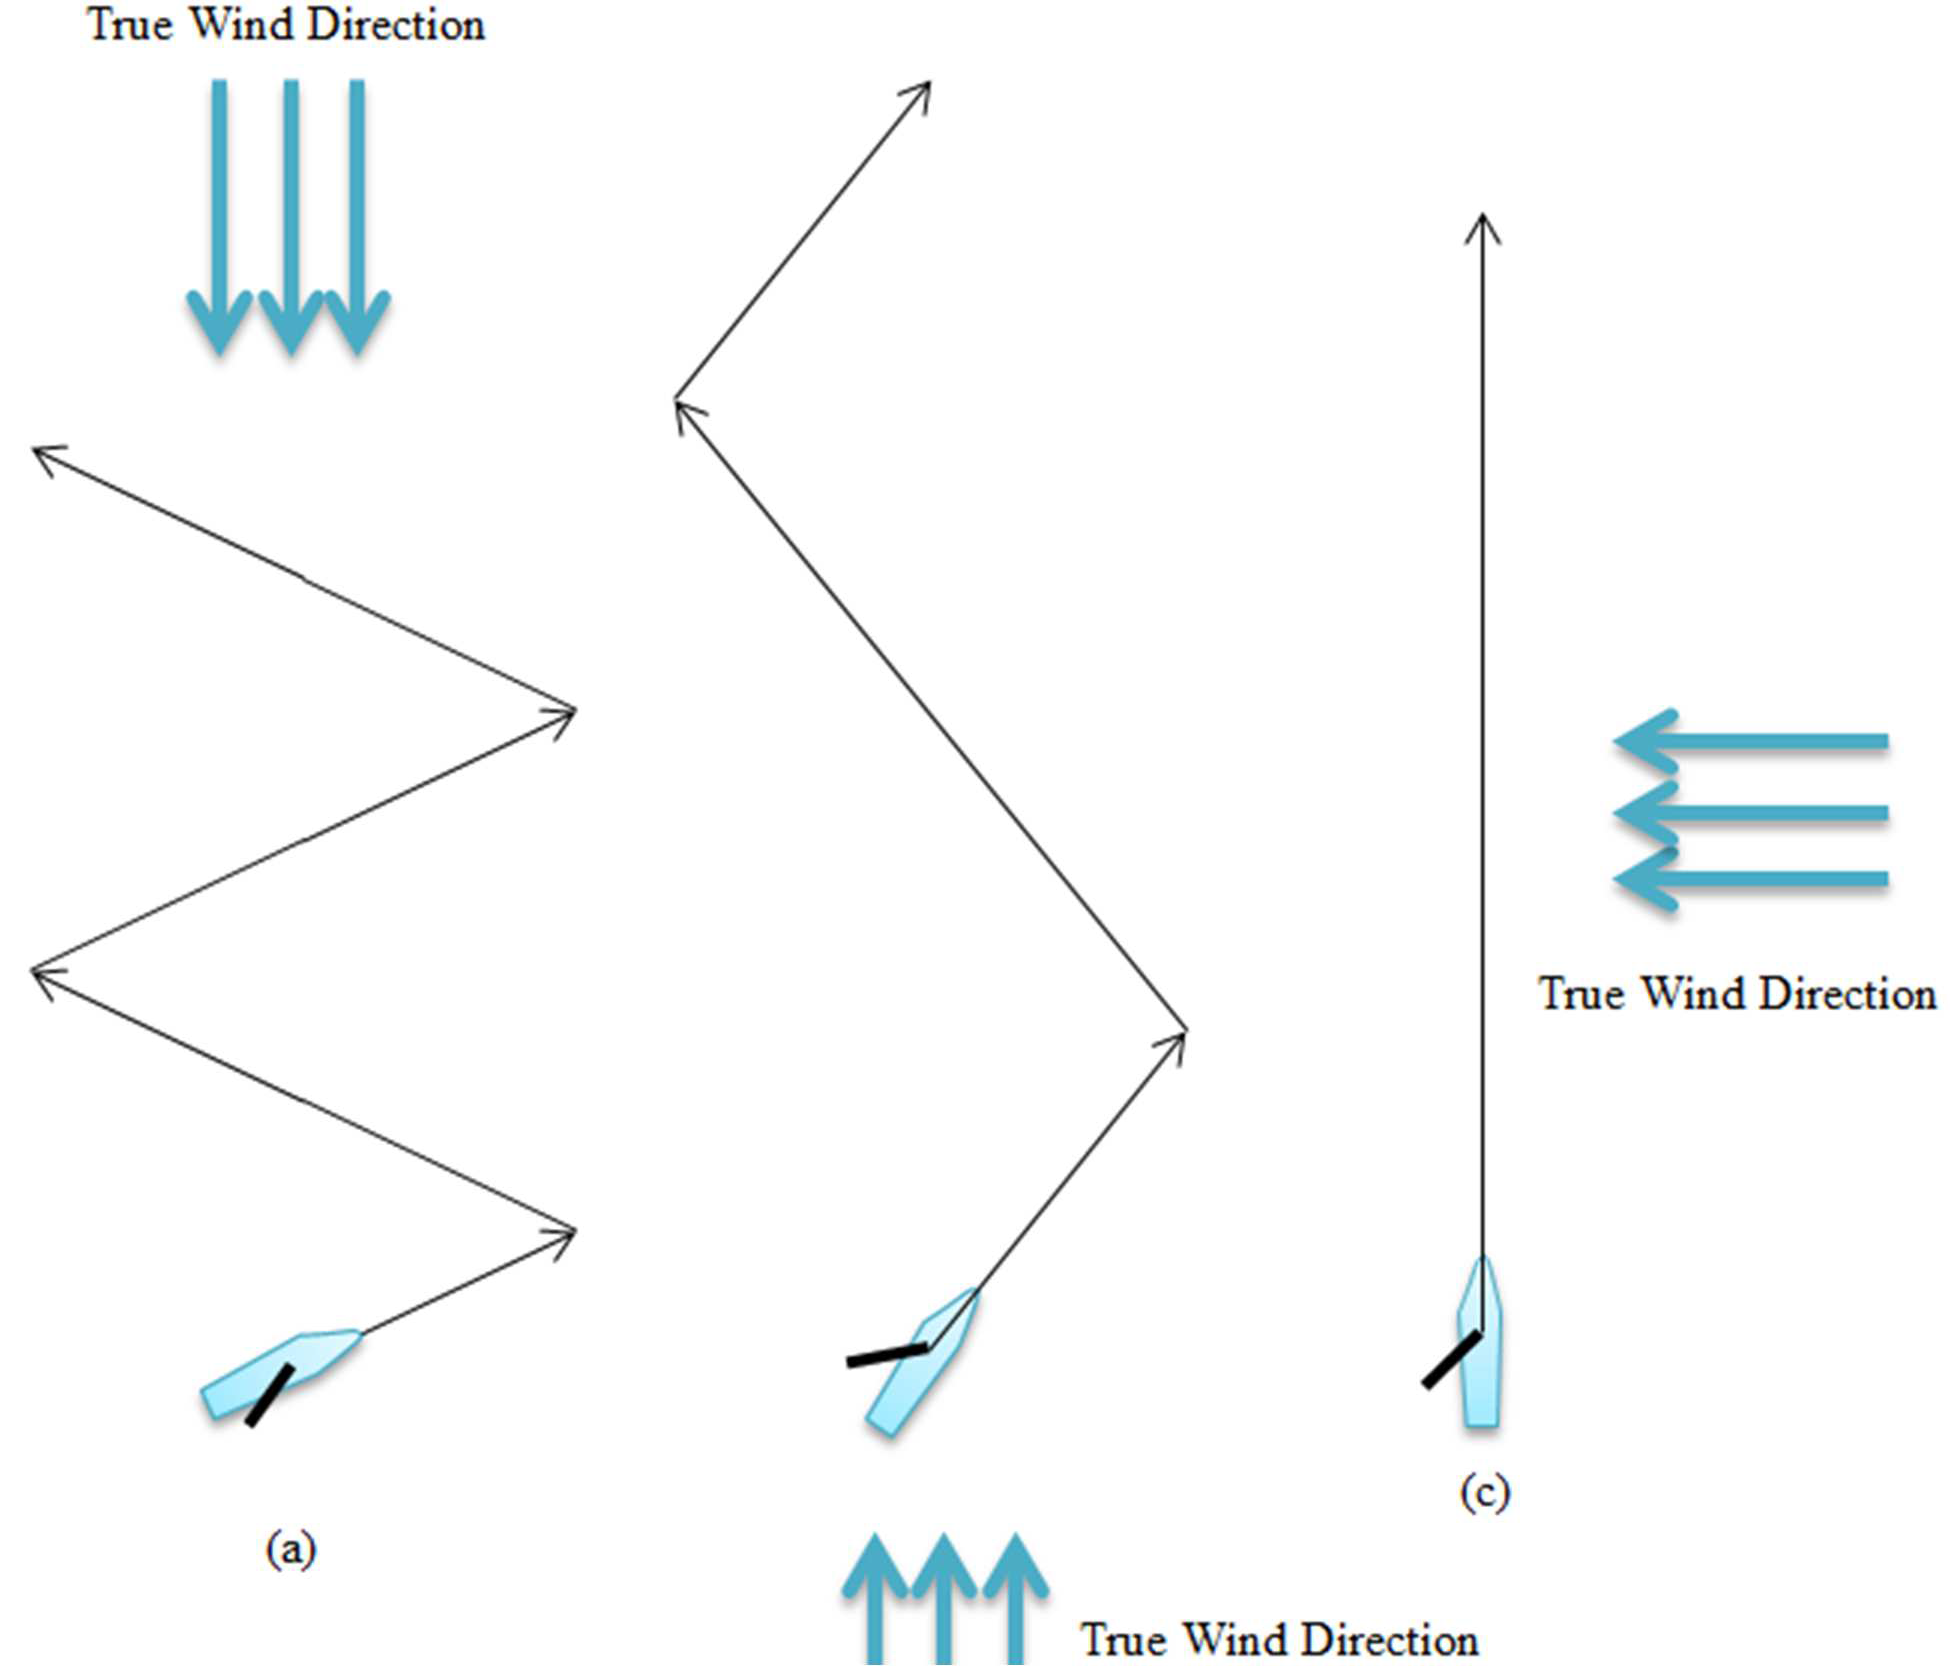
\includegraphics[width=\linewidth]{documents/figures/alves_modes.png}
    \caption{Modes of sailing \cite{Alves2010}}
    \label{fig:alves_modes}
\end{figure}
\column{0.5\linewidth}
\begin{figure}
    \centering
    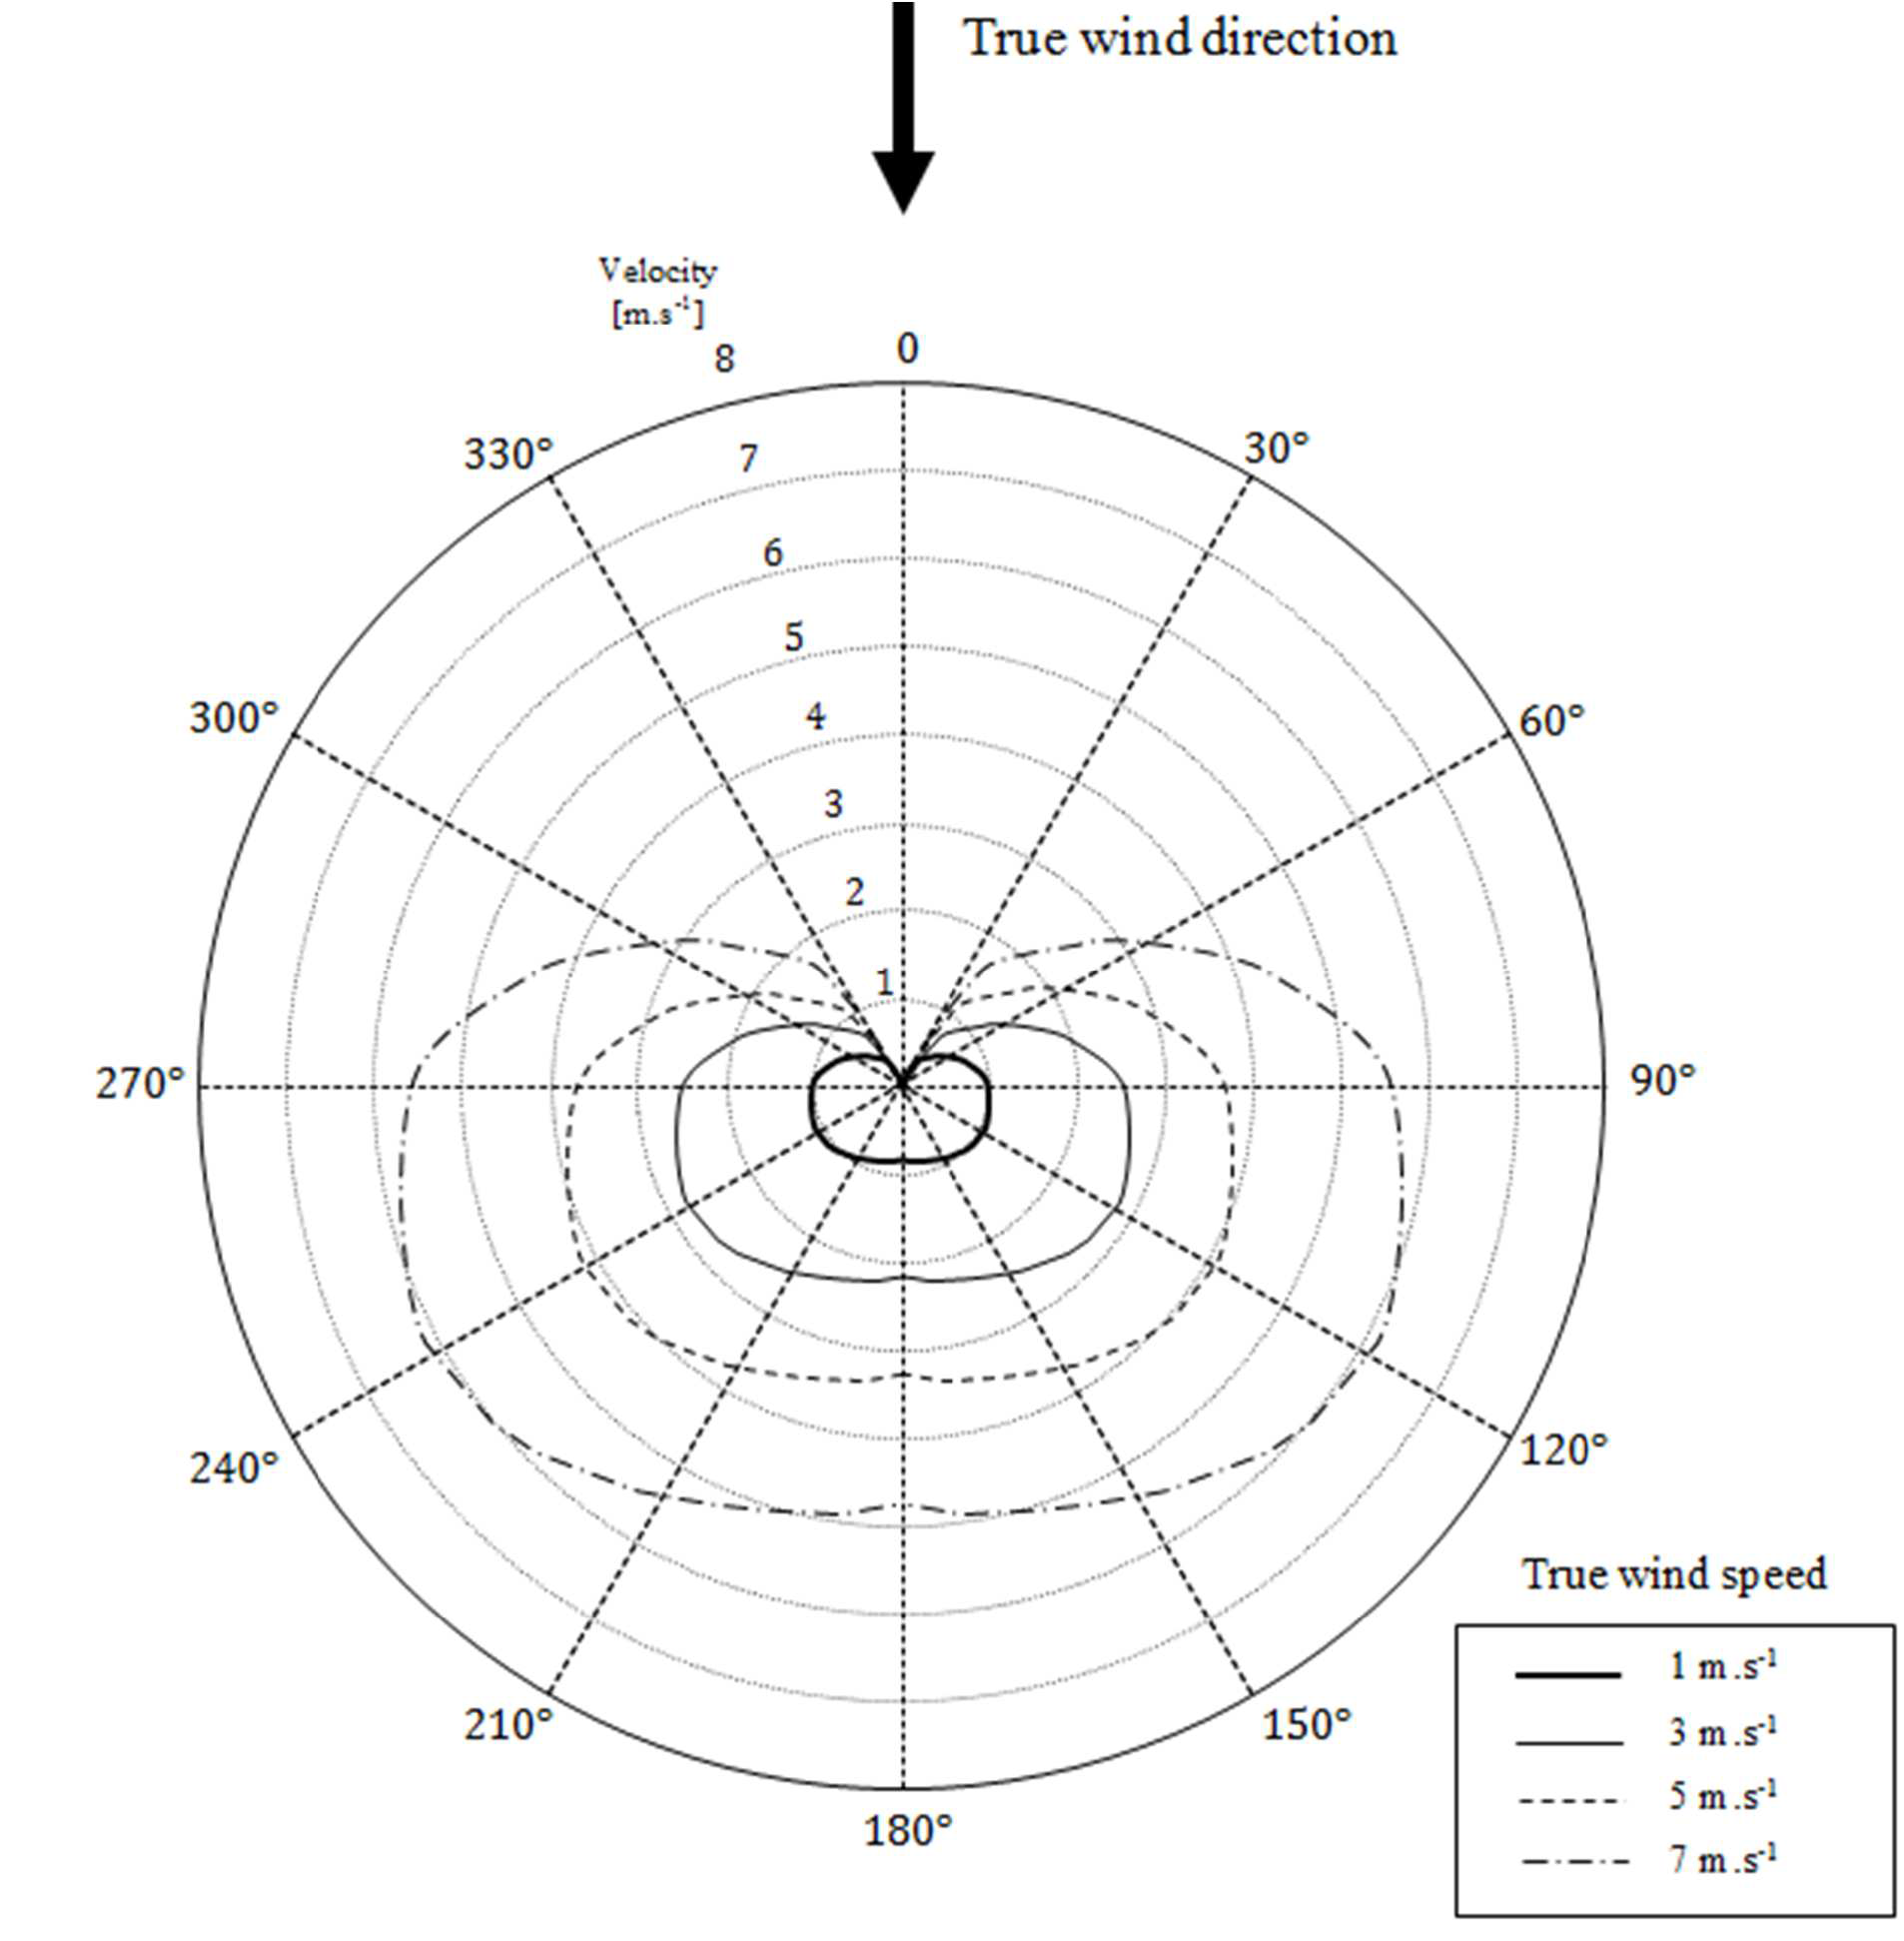
\includegraphics[width=\linewidth]{documents/figures/alves_vpp.png}
    \caption{Velocity polar diagram \cite{Alves2010}}
    \label{fig:alves_velocity}
\end{figure}
\end{columns}
\centerline{Sailboats trajectories depend on wind direction}
\end{frame}

\subsection{Sailboat model}

\begin{frame}{Sailboat Components}
\begin{columns}
\column{0.5\linewidth}
    \begin{figure}
        \centering
        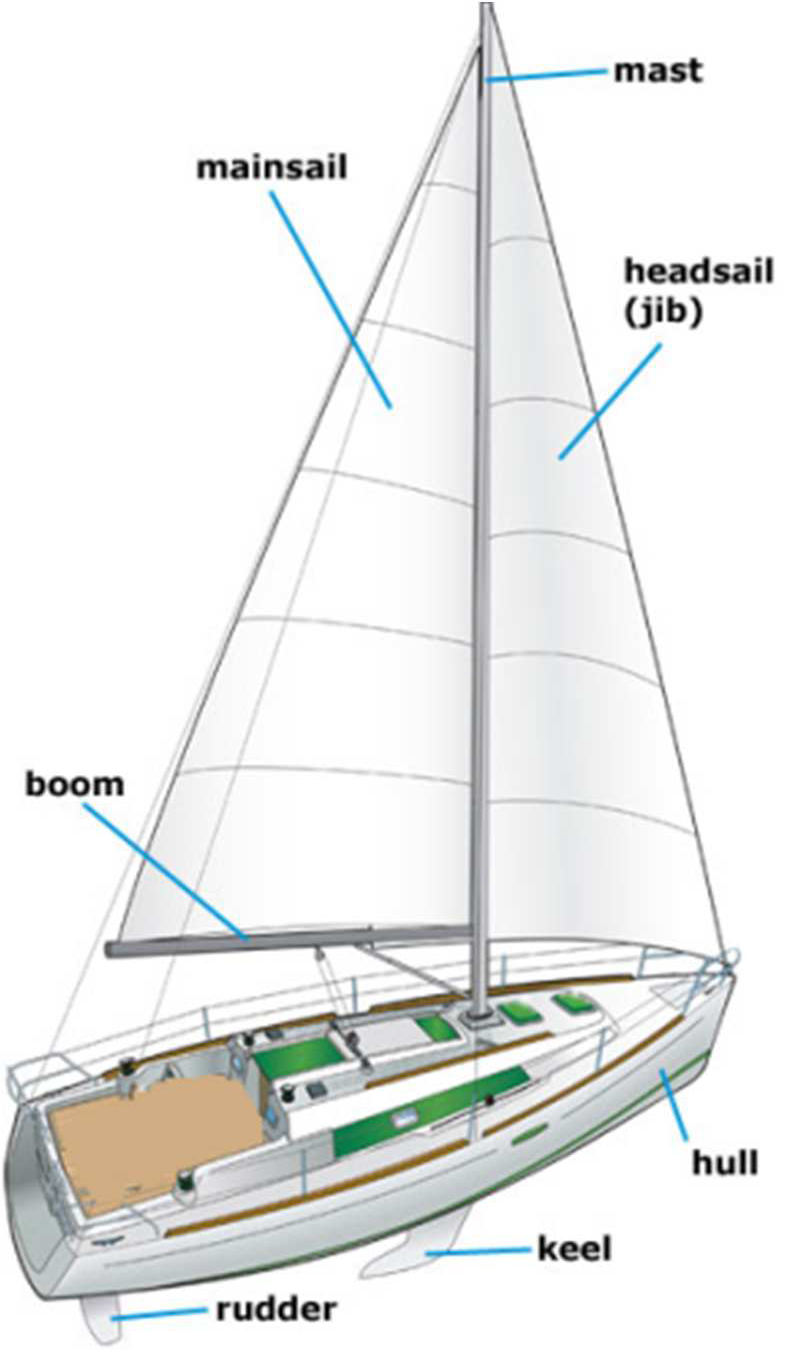
\includegraphics[height = 0.6\textheight, keepaspectratio]{documents/figures/alves_sailboat.png}
        \caption{Sailboat main components~\cite{Alves2010}.}
        \label{fig:my_label}
    \end{figure}
\column{0.5\linewidth}
\begin{itemize}
    \item Note that headsail and mainsail are connected in our model for simplicity
    \item Two control surfaces: sail and rudder \(\implies\) two actuators
\end{itemize}
\end{columns}

\end{frame}

\begin{frame}{6-DoF Model Axes}
\begin{columns}
\column{0.5\linewidth}
\begin{figure}
    \centering
    \includegraphics[width = \linewidth, height = \textheight, keepaspectratio]{documents/figures/alves}
    \caption{Sailboat axes~\cite{Alves2010}}
    \label{fig:my_label}
\end{figure}
\column{0.5\linewidth}
\begin{itemize}
    \item  \(X_B\)-\(Y\)-\(z\) translation
    \item Roll \-pitch-yaw rotation
\end{itemize}
\end{columns}

    
\end{frame}




\section{Simulator}
\begin{frame}{Evaluating Simulators}
    
    
    Simulators for sailboat models are significantly underdeveloped.
    
    \begin{columns}
    \column{0.5\linewidth}
        \centerline{\texttt{USVSim} \cite{Paravisi2019}}
        \begin{itemize}
            \item Ubuntu 16.04 + Kinetic ROS + Gazebo
            \item 6 DoF boat dynamics model.
            \item Waves, buoyancy, water currents, wind currents, thruster underwater, thruster above water, foil
            \item Too complicated to work with, hard to extend
        \end{itemize}
    \column{0.5\linewidth}
        \centerline{\texttt{stda-sailboat-sim} \cite{Buehler2018}}
        \begin{itemize}
            \item Python + Numpy + Matplotlib
            \item 6 DoF boat dynamics model.
            \item Waves, buoyancy, wind, sail, keel, rudder forces.
            \item Good enough 
        \end{itemize}
    \end{columns}
    
\end{frame}



\begin{frame}{Refactoring Simulator}

    \texttt{stda-sailboat-sim} simulator appears to have been written just enough to satisfy the needs of the authors paper.
    
    \hfill\\
    We rewrote it significantly to modularize the code and allow easy and structured definition
    of controllers and path planners.

\end{frame}

% \begin{frame}{Simulation Results}
% \begin{table}[h]
%     \centering
%     \begin{tabular}{lcc}
%     x-y trajectory & 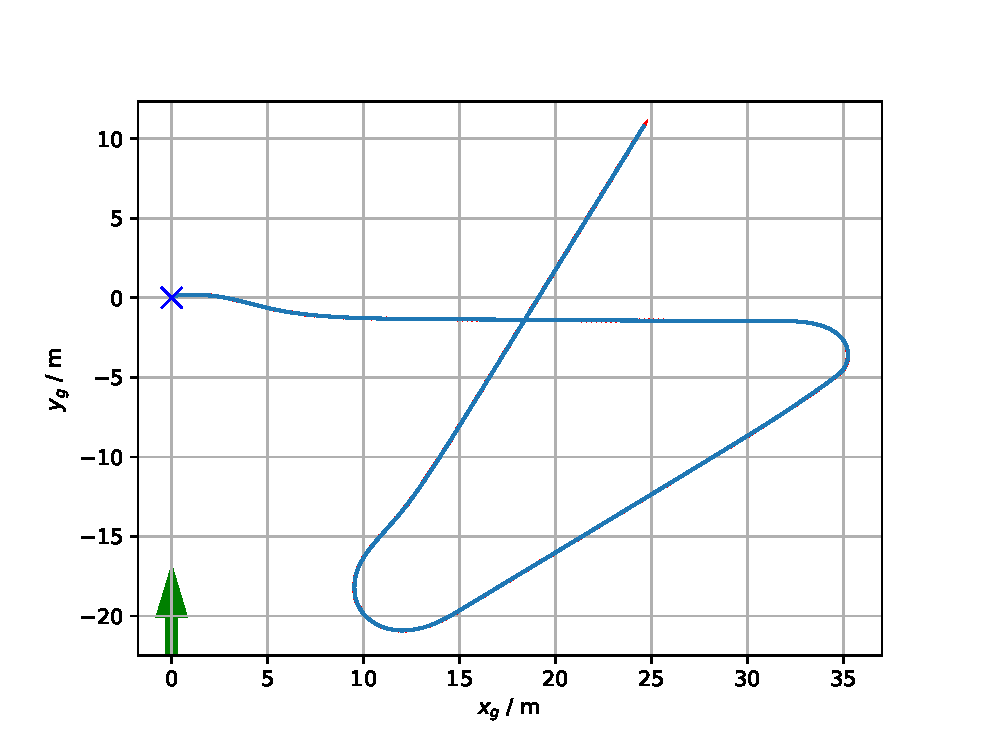
\includegraphics[width = 0.35\linewidth]{documents/figures/trajectories.eps} &
%     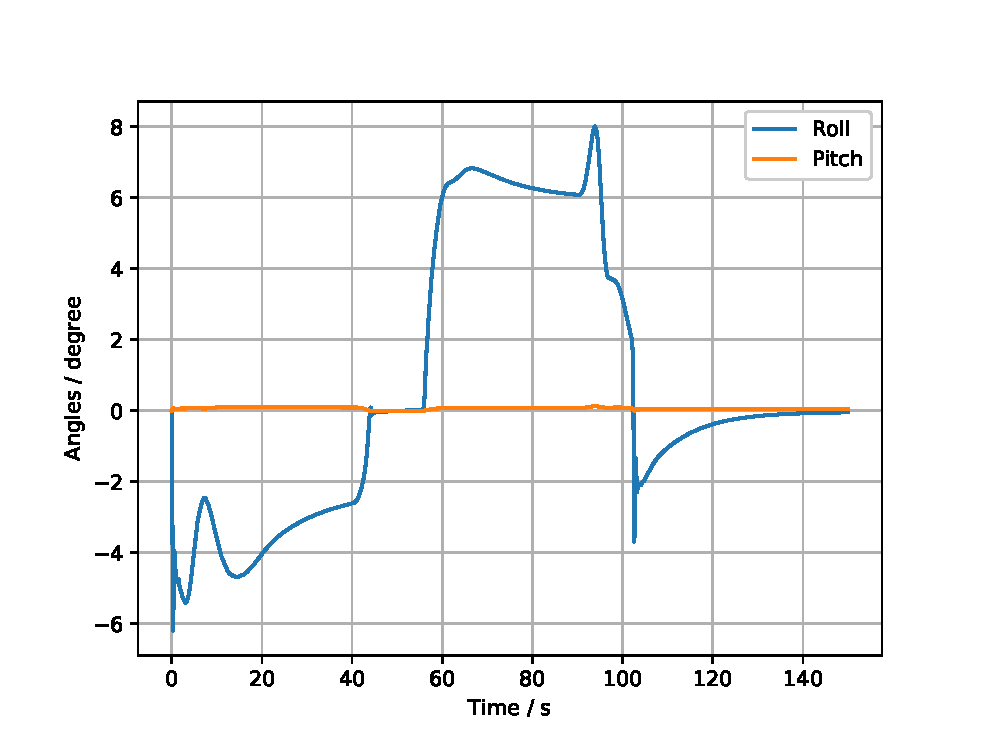
\includegraphics[width = 0.35\linewidth]{documents/figures/angles.eps} \\
%     heading angle & 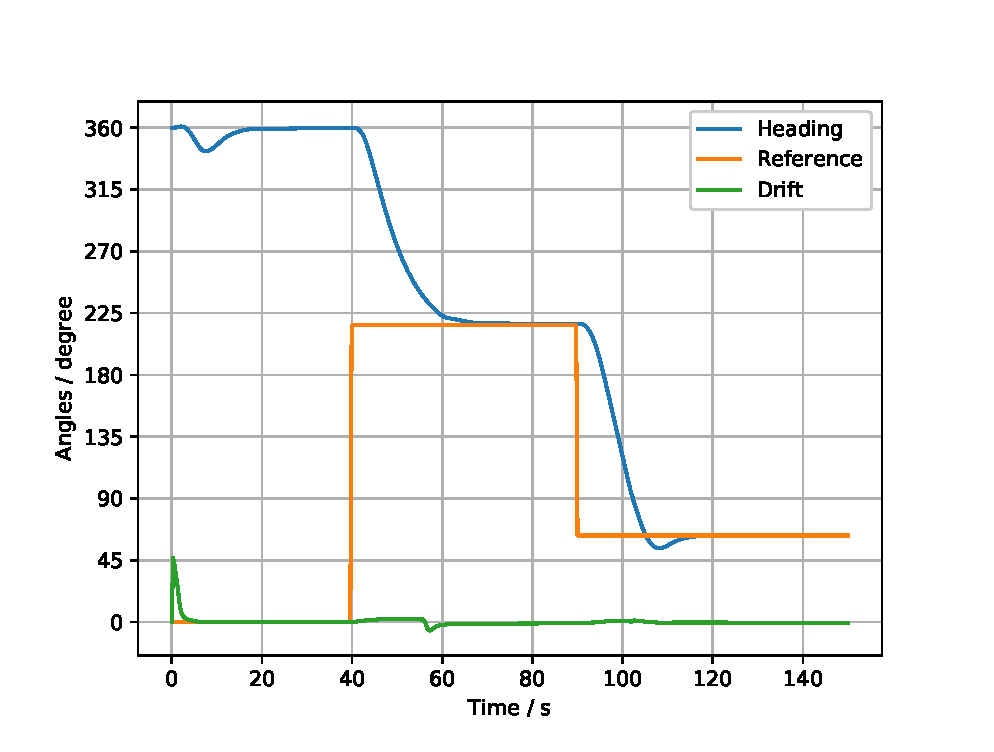
\includegraphics[width = 0.35\linewidth]{documents/figures/heading.eps} & 
%     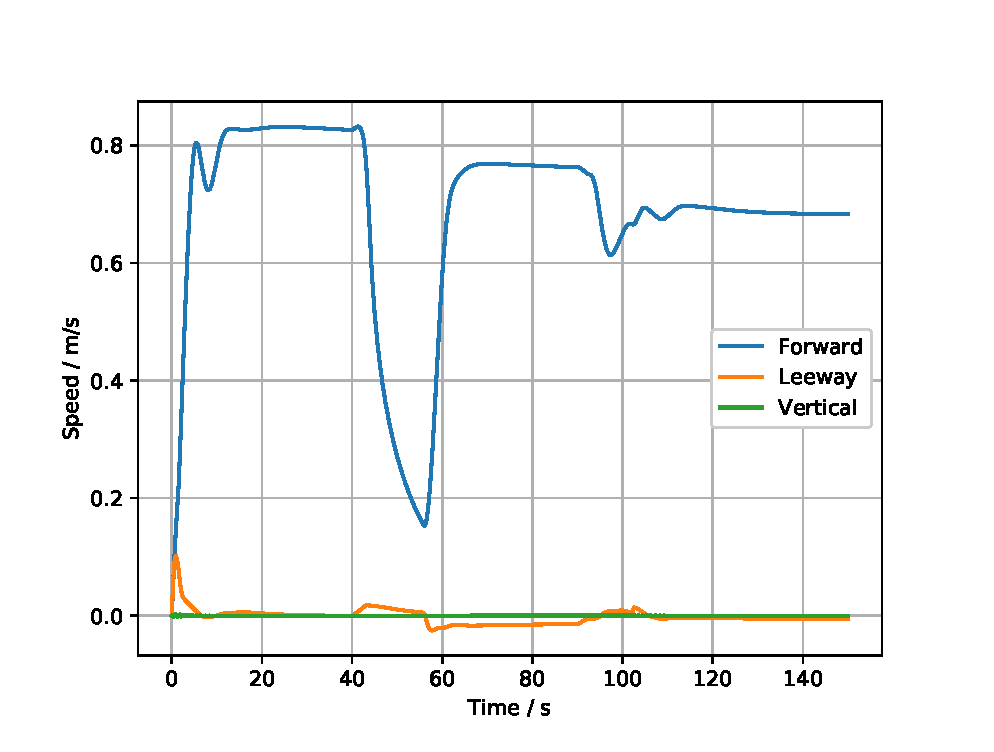
\includegraphics[width = 0.35\linewidth]{documents/figures/speeds.eps}
%     \end{tabular}
%     \caption{Simulator results with example reference headings}
%     \label{tab:plots  }
% \end{table}
% \end{frame}


\section{Control Design}

\begin{frame}{High-level Control Design}

\begin{figure}
    \centering
    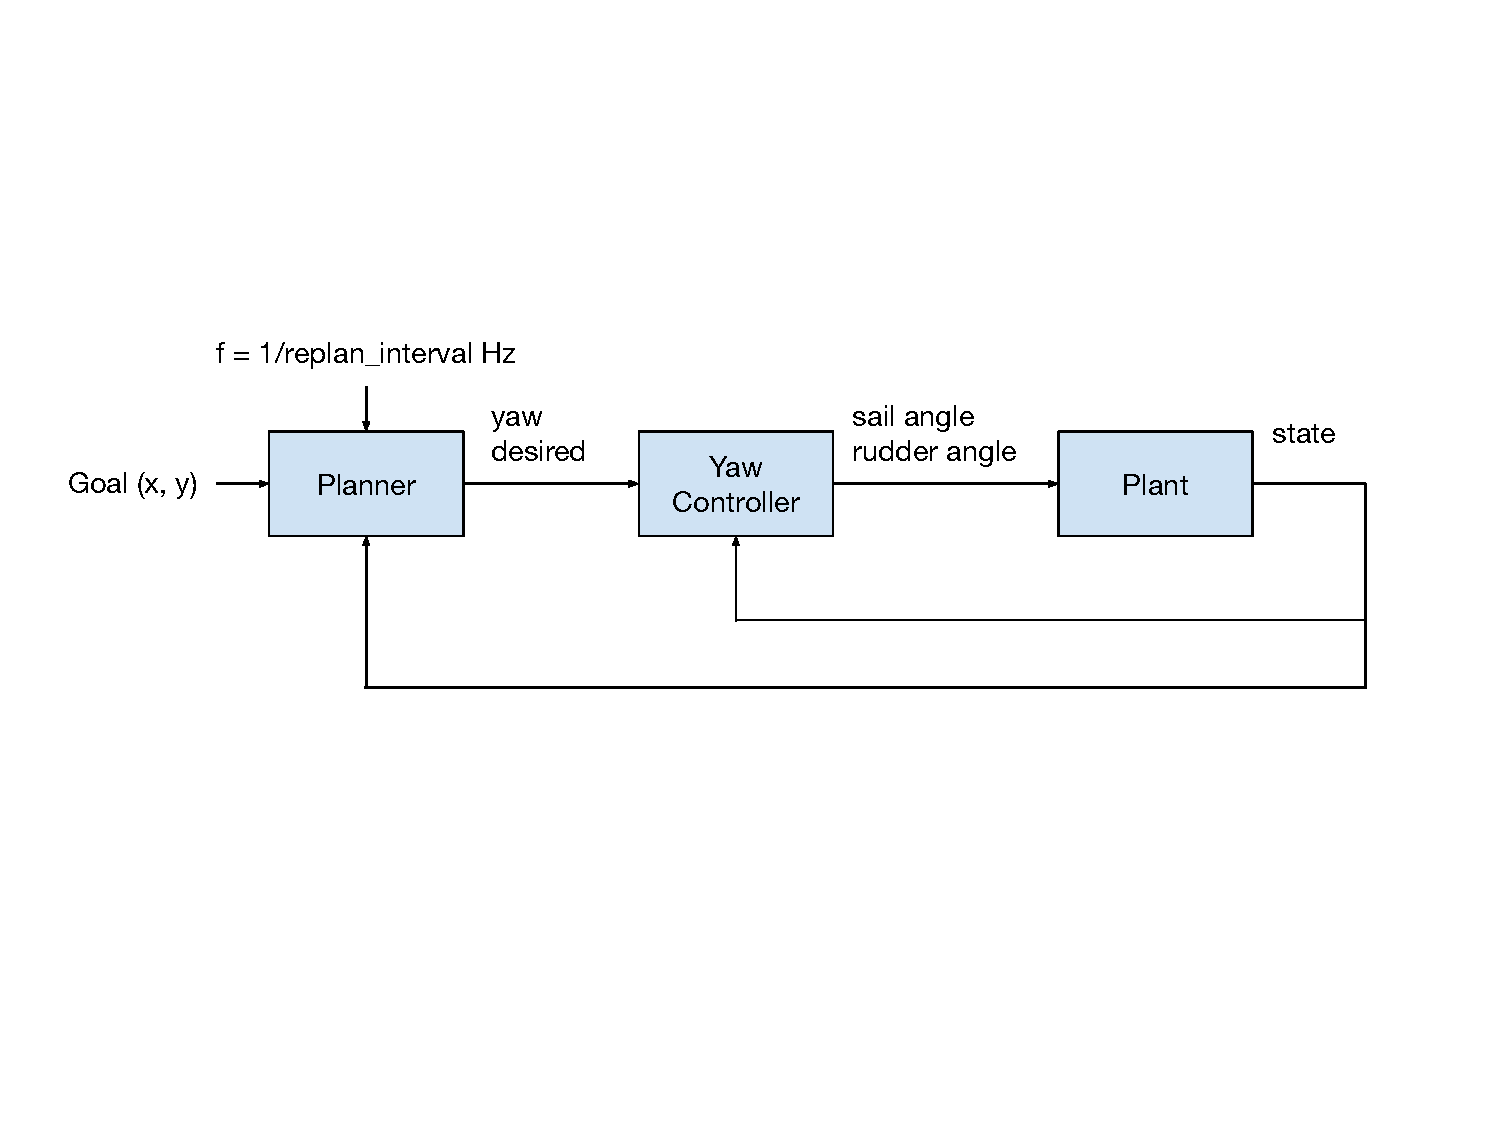
\includegraphics[width=\linewidth,trim={1cm 7cm 2cm 5cm},clip]{documents/final_pres_figs/controller_block_diagram.pdf}
    \caption{Block diagram of planner and controller}
    \label{fig:controller_block_diagram}
\end{figure}
    
A planner generates a reference heading (yaw) for the boat to reach a given \(x, y\) coordinate goal
and boat state.
The planner is run at a low rate since planning, and also the boat itself, is slow.

\hfill\\
The yaw controller generates sail angles and rudder angles to be used as inputs to the boat to
track the reference heading.

\end{frame}

\begin{frame}{Yaw Controller}

    The yaw controller tracks a reference yaw by setting sail and rudder angles.

    \hfill\\
    The yaw controller is implemented as per the same paper which developed the simulator and 
    boat dynamics model we are using\cite{Buehler2018}.
    
    \hfill\\
    This controller leverages the fact that there is an optimal angle for the sail based on wind direction to decouple the rudder and sail angle control.
    
    \hfill\\
    Note that the inputs called here as `rudder angle' and `sail angle' are actually
    inputs to a first order model that simulates delays in changing the rudder and sail angles,
    which are actually boat state variables.
    
    \hfill\\
    
    
\end{frame}

\begin{frame}{Yaw Controller}

    Apparent wind is the wind relative to the boat (accounting for boat velocity).
    
    \hfill\\
    With \(\theta_{aw}\) being the angle of the apparent wind, sail angle is optimally set based on current boat yaw as 
    \begin{equation}
        \theta_{\text{sail}} = \frac{\sin(\theta_{aw})}{\cos(\theta_{aw}) + 0.4\cos^2(\theta_{aw})}
    \end{equation}
    This is clipped based on sailboat limit.

    \hfill\\
    The rudder controller is implemented as a PID controller derived from a Jacobian linearization of a simplified dynamics model from input rudder to output yaw.
    
    \hfill\\
    Gains are determined through LQR.
    
\end{frame}

\begin{frame}{Planner}
    
    The planner takes in a high level \(x, y\) goal and plans a yaw trajectory for the boat 
    to reach the goal.
    
    \hfill\\
    We design the planner as repeatedly solving constrained nonlinear optimization problems with receding horizons. Due to model complexity, the planner runs slowly and so we define a 
    replanning interval on the order of 10s of seconds.
    
    \hfill\\
    Objective: the standard LQR-like quadratic objective with \(Q\) and \(R\) tunable cost matrices.
    
    \hfill\\
    Constraints: planned path must satisfy simplified boat dynamics and avoid obstacles.
    
    \hfill\\
    The optimization problems are solved with Casadi and the IPOPT solver.
    
\end{frame}

\begin{frame}{Planner: Boat Model}

    A simplified boat dynamics model is used in the planner to speed up planning.
    Also, some information used by the boat dynamics model are not well known 
    ahead of time.
    
    \hfill\\
    We make a simplified 3 state boat dynamics model with states \(x, y, \psi\) where 
    \(x, y\) are position and \(\psi\) is heading, and a non-physical input \(u\) 
    such that 
    
    \begin{equation}
        \mqty[\dot{x} \\ \dot{y} \\ \dot{\psi}]
         = \mqty[v_x \cos(\psi) - v_y \cos(\psi) \\ 
         v_x \sin(\psi) + v_y\cos(\psi) \\ 
         u]
    \end{equation}
    Why set yaw as integral of input instead of input itself?
    \begin{itemize}
        \item Ensures yaw is continuous.
        \item Allows limiting rate of change of yaw, ensuring planned path can be tracked.
    \end{itemize}

\end{frame}

\begin{frame}{Planner: Boat Model}
    Limitations of this boat model:
    \begin{itemize}
        \item Velocity model is severely simplified.
            \begin{itemize}
                \item We model \(v_x\) and \(v_y\) as constant over the planning horizon and equal to the velocities at the time of planning.
                \item Attempts at more detailed models such as setting speed as a cardioid based on difference between yaw and wind direction resulted in optimization failing to solve.
            \end{itemize}
        \item Model accuracy depends significantly on relative angle between wind and boat heading.
        \begin{itemize}
            \item Planner sometimes plans infeasible paths when going against wind.
        \end{itemize}
    \end{itemize}
    
    \hfill\\
    Replanning handles deviations from plan due to model mismatch and disturbances.
\end{frame}

\begin{frame}{Planner: Obstacles}

\end{frame}

\section{Experiments and Results}

\section{Conclusion}

\begin{frame}{Future Work and Improvements}

\begin{itemize}
    \item Simplified planner boat dynamics model:
\end{itemize}
    
\end{frame}

\begin{frame}{Conclusion}
    
\end{frame}

\begin{frame}{Thank You}
    Questions?
\end{frame}


\begin{frame}{References}
    \printbibliography{}
\end{frame}

\end{document}